\documentclass[class=article,crop=false]{standalone}

\usepackage{../setting/preamble_}

\begin{document}
\twocolumn
\section{Methodology}
\begin{center}
    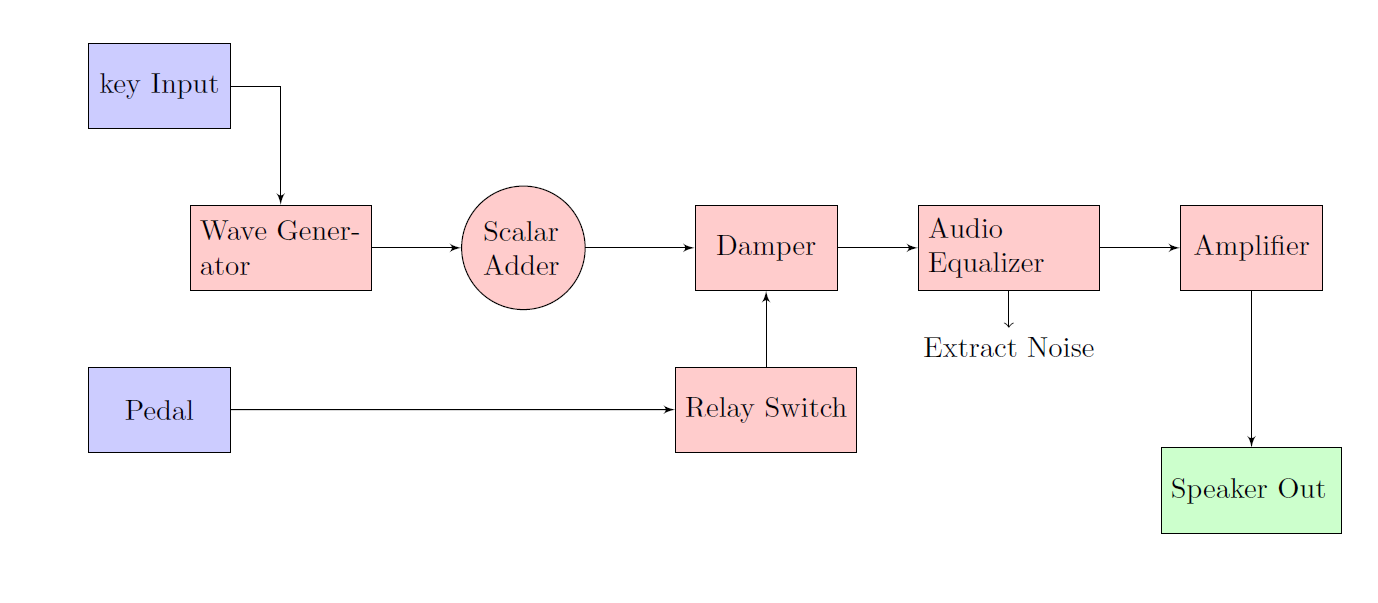
\includegraphics[width=.45\textwidth]{flow.png}
\end{center}

\subsection{Amplifier}
\subsubsection*{Class-A }
These are the simplest configuration among other families. It uses a single-ended transistor for its output stage with the resistive load connected directly to the Collector terminal. When the transistor switches “ON” it sinks the output current through the Collector resulting in an inevitable voltage drop across the Emitter resistance thereby limiting the negative output capability.  The current handling capability of such an amplifier family can be increased drastically by replacing the output transistor with \textbf{Darlington pair}. These devices provide high input impedance.
\begin{figure}
    \begin{center}
        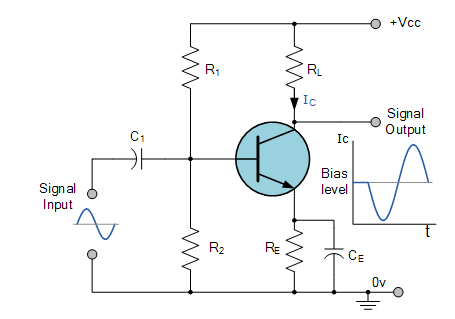
\includegraphics[width=.3\textwidth]{classA.png}
        \caption*{sdfsd}
    \end{center}
\end{figure}
\end{document}